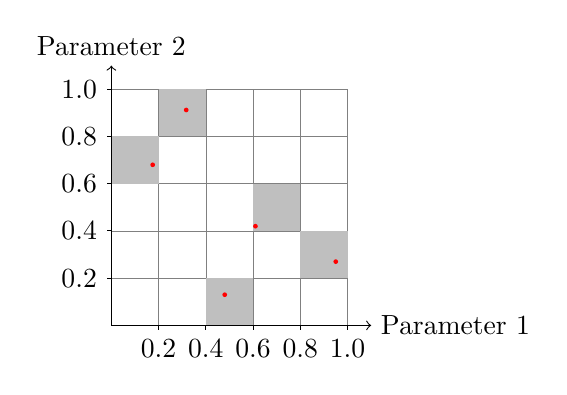
\begin{tikzpicture}[scale=3]

    % Define the grid
    \draw[step=0.2,gray,very thin] (0,0) grid (1,1);
    
    % Shade specific squares
    \fill[gray!50] (0.0,0.6) rectangle (0.2,0.8);
    \fill[gray!50] (0.2,0.8) rectangle (0.4,1.0);
    \fill[gray!50] (0.4,0.0) rectangle (0.6,0.2);
    \fill[gray!50] (0.6,0.4) rectangle (0.8,0.6);
    \fill[gray!50] (0.8,0.2) rectangle (1.0,0.4);
    
    % Draw red points
    \fill[red] (0.175,0.68) circle (0.01);  % Point in the first square
    \fill[red] (0.317,0.912) circle (0.01);  % Point in the second square
    \fill[red] (0.48,0.13) circle (0.01);  % Point in the third square
    \fill[red] (0.61,0.42) circle (0.01);  % Point in the fourth square
    \fill[red] (0.95,0.27) circle (0.01);  % Point in the fifth square
    
    % Draw the axes
    \draw[->] (0,0) -- (1.1,0) node[right] {Parameter 1};
    \draw[->] (0,0) -- (0,1.1) node[above] {Parameter 2};
    
    % Add ticks and labels
    \foreach \x in {0.2,0.4,0.6,0.8,1.0} {
      \draw (\x,0) -- (\x,-0.02) node[below] {\x};
      \draw (0,\x) -- (-0.02,\x) node[left] {\x};
    }
    
\end{tikzpicture}